\documentclass[11pt, oneside]{article}   	% use "amsart" instead of "article" for AMSLaTeX format
\usepackage{geometry}                		% See geometry.pdf to learn the layout options. There are lots.
\geometry{letterpaper}                   		% ... or a4paper or a5paper or ... 
%\geometry{landscape}                		% Activate for for rotated page geometry
%\usepackage[parfill]{parskip}    		% Activate to begin paragraphs with an empty line rather than an indent
\usepackage{graphicx}				% Use pdf, png, jpg, or eps with pdflatex; use eps in DVI mode
								% TeX will automatically convert eps --> pdf in pdflatex		
\usepackage{amssymb}
\usepackage{amsmath}

\newcommand{\HRule}{\rule{\linewidth}{0.5mm}}

\title{A Two-Mass Oscillator}
\setlength\parindent{0pt}

\begin{document}

\begin{titlepage}
		\begin{center}
			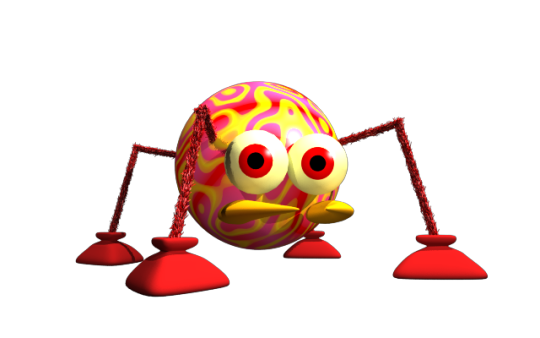
\includegraphics[scale=0.2]{logo}\\[1cm]
			
			\textsc{\LARGE MAT 485 Project 1}\\[2cm]
			\textsc{\Large Cal Poly Pomona}\\[1cm]
			
		
			\HRule \\[0.4cm]
			{\huge \bfseries A Two-Mass Oscillator \\[0.4cm]}
			\HRule \\[2cm]
			
			\noindent
			\begin{minipage}{0.4\textwidth}
				\begin{flushleft}
					\large
					\emph{Authors:}\\
					Morgan Rupard \\ Aaron Gaut
				\end{flushleft}
			\end{minipage}
			\begin{minipage}{0.4\textwidth}
				\begin{flushright}
					\large
					\emph{Professor:}\\
					Dr. Jennifer Switkes
			\end{flushright}
			\end{minipage}
			
			\vfill
			
			{\large February $19^{\text{th}}$, 2016}
		\end{center}
	\end{titlepage}

\tableofcontents
\newpage

\section{Introduction}
In this paper we will model the two-mass oscillator system.
Consider the diagram shown in Figure~\ref{sketch}.

\begin{figure}[h!]
\centering 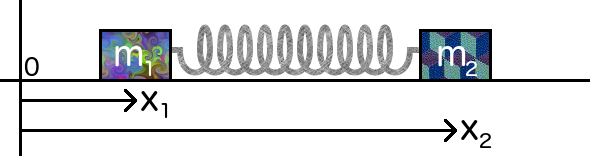
\includegraphics[scale=0.7]{sketch}
\caption{\label{sketch} The two-mass oscillator system}
\end{figure}

In this system there are two masses attached horizontally by a spring.
We will explore the scenario in which the spring's force is governed by Hooke's Law.
We will use a coordinate system relative to an arbitrary fixed origin.
The first object has mass $m_1$ and is positioned at $x_1$.
For the second mass, $m_2$ and $x_2$ are defined similarly.
The spring constant is determined by the parameter $k$, and the unstretched length of the spring is $L$.

The displacement by which the spring is stretch is given by $x_2 - x_1 -L$.
Therefore, by Hooke's Law, we can determine the acceleration of each mass,
\begin{align*}
m_1 \frac{d^2x_1}{dt^2} &= k(x_2 - x_1 - L), \\
m_2 \frac{d^2x_2}{dt^2} &= -k(x_2 - x_1 - L). \\
\end{align*}

From here, the following can be shown:
\begin{align}
&\frac{d^2}{dt^2}(m_1x_1 + m_2x_2) = 0, \\
&\frac{d^2z}{dt^2} = -k\left(\frac{1}{m_1}+\frac{1}{m_2}\right)z \text{, \;where } z = x_2-x_1-L,
\end{align}

In the following sections we will assume these initial conditions:
$$\begin{matrix}
x_1(0) = \alpha, & \dfrac{dx_1}{dt}(0) = \gamma, \\ &\\
x_2(0) = \beta, & \dfrac{dx_2}{dt}(0) = \delta.
\end{matrix}$$
\section{Analytical Work}
We will now solve equation (1) analytically by integrating twice.
\begin{align*}
&\frac{d^2}{dt^2}(m_1x_1 + m_2x_2) = 0 \\
\implies & \frac{d}{dt}(m_1x_1 + m_2x_2) = C\\
\implies & m_1x_1 + m_2x_2 = Ct+D,
\end{align*}
for constants of integration $C$ and $D$. Now we impose the initial conditions.
We have the system of equations,
\begin{align*}
m_1\alpha + m_2\beta &= D, \\
m_1\gamma + m_2\delta &= C,
\end{align*}
and thus,
\begin{equation}
m_1x_1 + m_2x_2 = (m_1\gamma + m_2\delta)t + m_1\alpha + m_2\beta.
\end{equation}

Now, we will solve equation (2) using an eigenvalue approach.
If we do this then we will find that the roots of the characteristic polynomial are:

$$r = \pm \sqrt{k\left(\frac{1}{m_1}+\frac{1}{m_2}\right)}i$$

We will let $\displaystyle{\omega = \sqrt{k\left(\frac{1}{m_1}+\frac{1}{m_2}\right)}}$. This implies that the the general solution to equation (2) is:

$$z(t) = c_1\cos{(\omega t)}+c_2\sin{(\omega t)}$$

We will now impose the initial conditions in order to find $c_1$ and $c_2$.
We will also back-substitute $x_1$ and $x_2$ into the equation, which results in:

\begin{equation}
x_2-x_1-L = \left(\beta - \alpha - L\right)\cos{\left(\omega t\right)}+\frac{\delta - \gamma}{\omega}\sin{(\omega t)}
\end{equation}

\section{Numerical Work}
We used the MATLAB function \texttt{fsolve}, a nonlinear implicit equation solver, together with the analytically derived equations (3) and (4), to explore the system.
We also determined the center of mass with the formula
$$
x_{cm}(t) = \frac{m_1x_1(t) + m_2x_2(t)}{m_1 + m_2}.
$$

\subsection{Sanity Checks}
First we will verify our numerical work by testing with initial conditions that have intuitive outcomes.
For example if the initial conditions have symmetry then so should $x_1$ and $x_2$.
We tested this using the parameters
\begin{center}

\begin{tabular}{| c | c | c | c | c | c | c | c |}

\hline

$L$ & $\alpha$ & $\beta$ & $\gamma$ & $\delta$ & $m_1$ & $m_2$ & $k$ \\

\hline

 10 & 0 & 18 & 0 & 0 & 10 & 10 & 3\\

\hline

\end{tabular}

\end{center}

The notable parameters in this case are $\gamma, \delta, m_1, $ and $m_2$.
Both objects have zero initial velocity, and the objects have equal mass.
The result can be seen in Figure~\ref{sanity1}.
The two objects oscillate symmetrically, maintaining equal distance from the center of mass.
This matches our intuition.

\begin{figure}[h!]
\centering 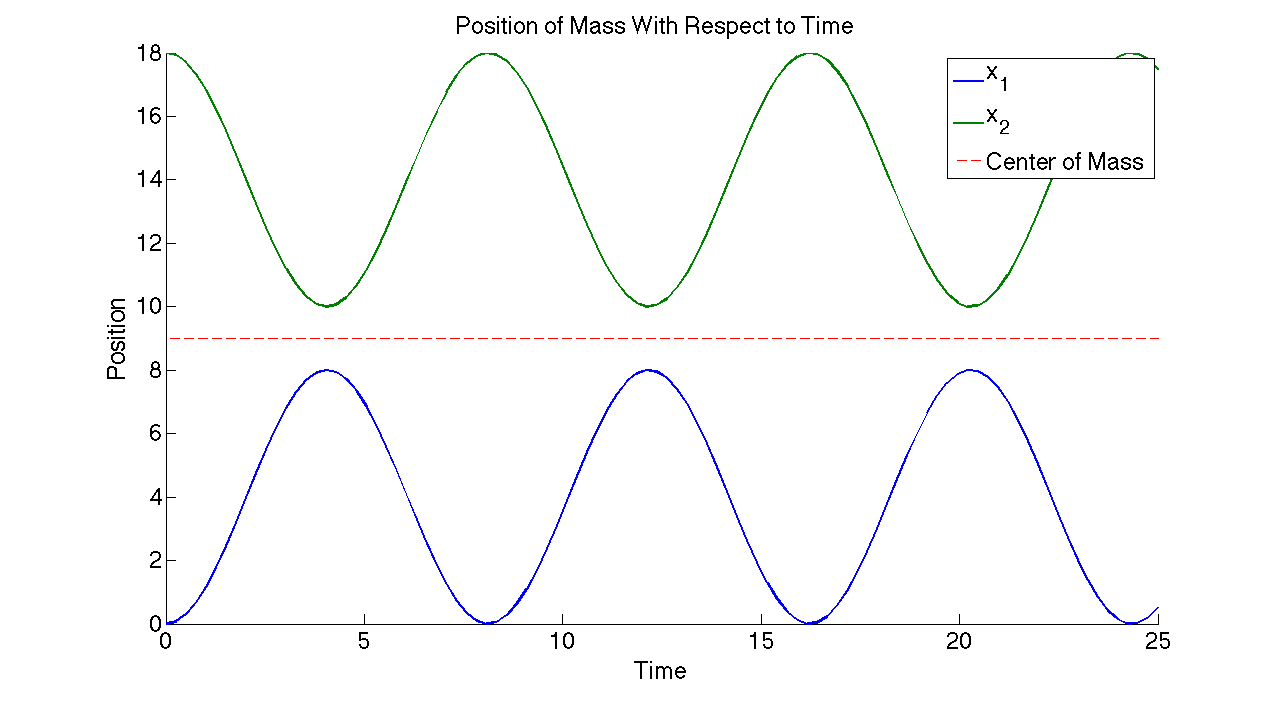
\includegraphics[scale=0.3]{sanity1}
\caption{\label{sanity1} Symmetric motion with zero initial velocity}
\end{figure}

Another predictable case to consider is one where the spring is initially at equilibrium ($\beta - \alpha - L = 0$), and the masses have equal initial velocity ($\delta-\gamma=0$).
Since both masses will slide in the same direction at the same speed, the spring will remain at equilibrium.
As long as the spring remains at equilibrium it will not apply force on either mass, and thus both masses will continue to slide with their initial velocity.
We tested this with the parameters

\begin{center}

\begin{tabular}{| c | c | c | c | c | c | c | c |}

\hline

$L$ & $\alpha$ & $\beta$ & $\gamma$ & $\delta$ & $m_1$ & $m_2$ & $k$ \\

\hline

 10 & 0 & 10 & 1 & 1 & 2 & 10 & 3\\

\hline

\end{tabular}

\end{center}

\begin{figure}[h!]
\centering 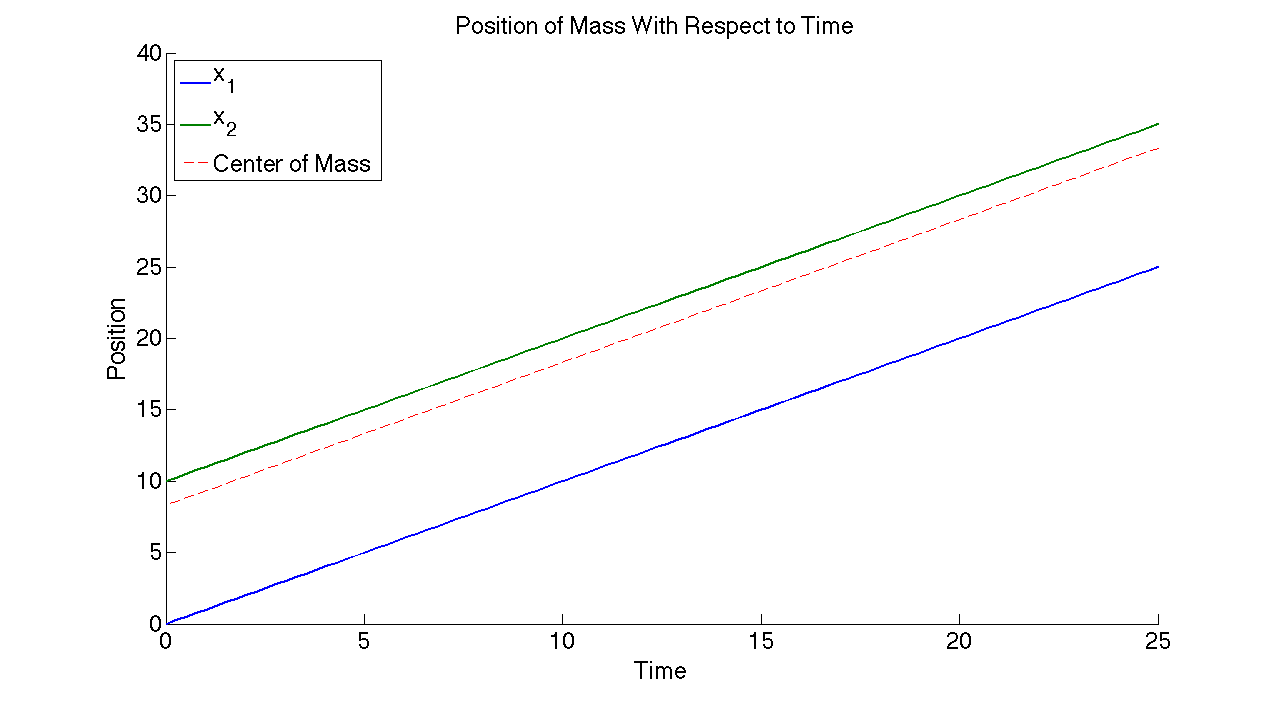
\includegraphics[scale=0.3]{sanity2}
\caption{\label{sanity2} The linear motion case}
\end{figure}

These parameters lead to the linear motion case.
The plot resulting from these parameters is shown in Figure~\ref{sanity2}.
The center of mass is also linear but closer to $x_2$ since $m_2$ is larger than $m_1$.
This set of initial conditions is interesting because its constraints,

\begin{align*}
\beta - \alpha - L &= 0,\\
\delta - \gamma &= 0,
\end{align*}

correspond to the initial conditions $z(0)=0$ and $\dfrac{dz}{dt}(0) = 0$.
Since $z$ obeys simple harmonic motion, this is the case where $z$ is constant 0.

\subsection{The Spring Singularity}
Consider a situation in which the two masses touch at a single point along the center of mass line periodically.
This is not physically possible because it implies that the spring has popped out of existence or has phased into the two masses.
Even though it is not possible it is still interesting to look at and makes a really pretty picture.
It turns out that it is a little bit difficult to find the correct constants for this to happen because we need the total maximum amplitude of each curve to be $L$, which would mean solving this equation for each constant:

$$\sqrt{(\beta - \alpha -L)^2 + \left(\frac{\delta - \gamma}{\omega}\right)^2}=L$$

This is incredibly difficult, but we can impose some requirements that makes this a simpler task such as making one of the terms under the square root $0$:

$$\delta - \gamma = 0 \implies \beta - \alpha = 2L$$

If we do this using the parameters

\begin{center}

\begin{tabular}{| c | c | c | c | c | c | c | c |}

\hline

$L$ & $\alpha$ & $\beta$ & $\gamma$ & $\delta$ & $m_1$ & $m_2$ & $k$ \\

\hline

 9 & 0 & 18 & 2 & 2 & 10 & 5 & 4\\

\hline

\end{tabular}

\end{center}

we then get a plot that looks like: \\

\begin{figure}[h!]
\centering 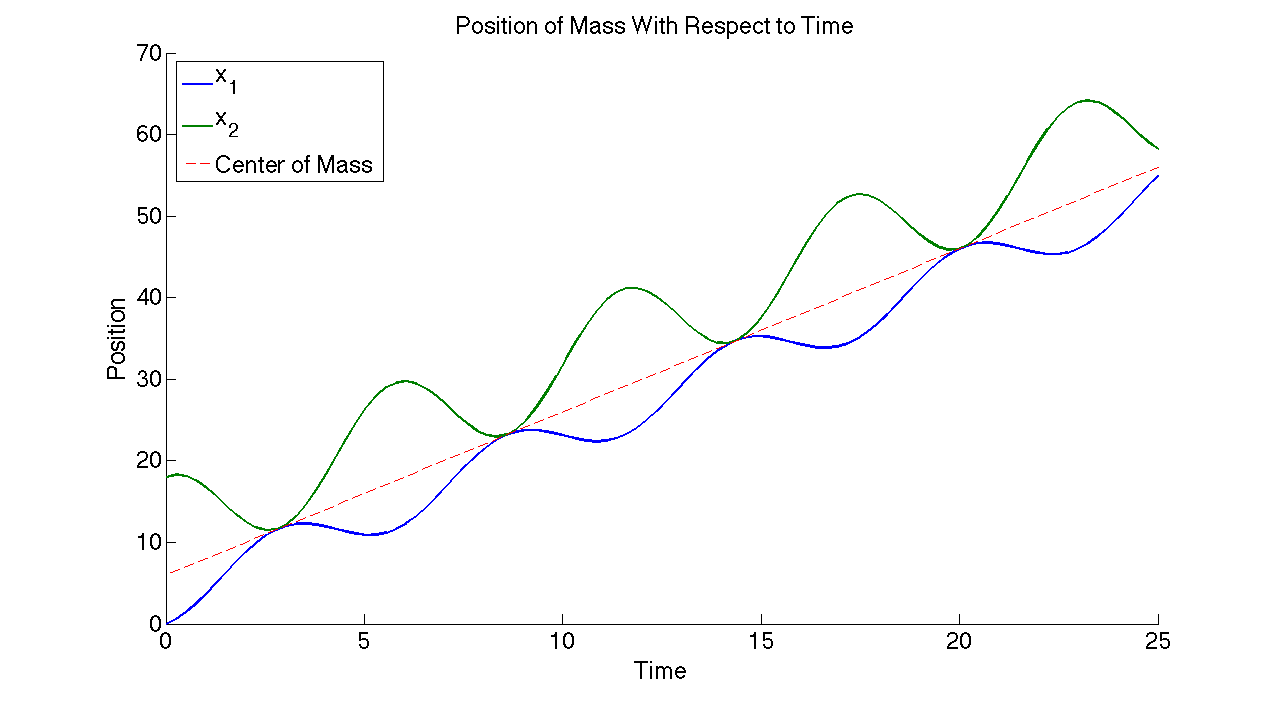
\includegraphics[scale=0.3]{spring_sing}
\caption{\label{singularity}One example of the spring singularity}
\end{figure}



\section{Discussion}

\section{Appendix}


\end{document}  
